% Options for packages loaded elsewhere
\PassOptionsToPackage{unicode}{hyperref}
\PassOptionsToPackage{hyphens}{url}
%
\documentclass[
]{article}
\usepackage{lmodern}
\usepackage{amsmath}
\usepackage{ifxetex,ifluatex}
\ifnum 0\ifxetex 1\fi\ifluatex 1\fi=0 % if pdftex
  \usepackage[T1]{fontenc}
  \usepackage[utf8]{inputenc}
  \usepackage{textcomp} % provide euro and other symbols
  \usepackage{amssymb}
\else % if luatex or xetex
  \usepackage{unicode-math}
  \defaultfontfeatures{Scale=MatchLowercase}
  \defaultfontfeatures[\rmfamily]{Ligatures=TeX,Scale=1}
\fi
% Use upquote if available, for straight quotes in verbatim environments
\IfFileExists{upquote.sty}{\usepackage{upquote}}{}
\IfFileExists{microtype.sty}{% use microtype if available
  \usepackage[]{microtype}
  \UseMicrotypeSet[protrusion]{basicmath} % disable protrusion for tt fonts
}{}
\makeatletter
\@ifundefined{KOMAClassName}{% if non-KOMA class
  \IfFileExists{parskip.sty}{%
    \usepackage{parskip}
  }{% else
    \setlength{\parindent}{0pt}
    \setlength{\parskip}{6pt plus 2pt minus 1pt}}
}{% if KOMA class
  \KOMAoptions{parskip=half}}
\makeatother
\usepackage{xcolor}
\IfFileExists{xurl.sty}{\usepackage{xurl}}{} % add URL line breaks if available
\IfFileExists{bookmark.sty}{\usepackage{bookmark}}{\usepackage{hyperref}}
\hypersetup{
  pdftitle={Model Results},
  pdfauthor={Xilin Chen},
  hidelinks,
  pdfcreator={LaTeX via pandoc}}
\urlstyle{same} % disable monospaced font for URLs
\usepackage[margin=1in]{geometry}
\usepackage{graphicx}
\makeatletter
\def\maxwidth{\ifdim\Gin@nat@width>\linewidth\linewidth\else\Gin@nat@width\fi}
\def\maxheight{\ifdim\Gin@nat@height>\textheight\textheight\else\Gin@nat@height\fi}
\makeatother
% Scale images if necessary, so that they will not overflow the page
% margins by default, and it is still possible to overwrite the defaults
% using explicit options in \includegraphics[width, height, ...]{}
\setkeys{Gin}{width=\maxwidth,height=\maxheight,keepaspectratio}
% Set default figure placement to htbp
\makeatletter
\def\fps@figure{htbp}
\makeatother
\setlength{\emergencystretch}{3em} % prevent overfull lines
\providecommand{\tightlist}{%
  \setlength{\itemsep}{0pt}\setlength{\parskip}{0pt}}
\setcounter{secnumdepth}{-\maxdimen} % remove section numbering
\usepackage{booktabs}
\usepackage{longtable}
\usepackage{array}
\usepackage{multirow}
\usepackage{wrapfig}
\usepackage{float}
\usepackage{colortbl}
\usepackage{pdflscape}
\usepackage{tabu}
\usepackage{threeparttable}
\usepackage{threeparttablex}
\usepackage[normalem]{ulem}
\usepackage{makecell}
\usepackage{xcolor}
\ifluatex
  \usepackage{selnolig}  % disable illegal ligatures
\fi

\title{Model Results}
\author{Xilin Chen}
\date{4/20/2021}

\begin{document}
\maketitle

\hypertarget{death-30days}{%
\subsection{Death 30days}\label{death-30days}}

\hypertarget{regression-table}{%
\subsubsection{Regression table}\label{regression-table}}

Fixed effect table

\begin{table}[H]
\centering
\begin{tabular}{l|r|r|r}
\hline
term & estimate & OR & p\_value\\
\hline
(Intercept) & -3.2284951 & 0.0396171 & 0.000\\
\hline
re\_cert\_binPassed & 0.0112347 & 1.0112980 & 0.447\\
\hline
flg\_male & 0.1264258 & 1.1347653 & 0.000\\
\hline
age\_at\_admit\_std & 0.3155463 & 1.3710081 & 0.000\\
\hline
AHRQ\_score\_std & 0.6310275 & 1.8795408 & 0.000\\
\hline
race\_white & 0.1243647 & 1.1324288 & 0.000\\
\hline
seslow\_ses & 0.1663321 & 1.1809652 & 0.000\\
\hline
emergent\_admit & 0.8655416 & 2.3762928 & 0.000\\
\hline
year & -0.0388332 & 0.9619112 & 0.000\\
\hline
surgeon\_yearly\_load\_std & 0.0011493 & 1.0011500 & 0.719\\
\hline
hospital\_icu & -0.0027460 & 0.9972578 & 0.891\\
\hline
hospital\_urban & -0.0534239 & 0.9479781 & 0.000\\
\hline
hospital\_beds\_gt\_350>350 & -0.0287827 & 0.9716276 & 0.000\\
\hline
hospital\_rn2bed\_ratio\_std & -0.0879210 & 0.9158332 & 0.000\\
\hline
hospital\_mcday2inptday\_ratio\_std & 0.0163292 & 1.0164632 & 0.000\\
\hline
\end{tabular}
\end{table}

\hypertarget{fig1}{%
\subsubsection{Fig1}\label{fig1}}

\begin{center}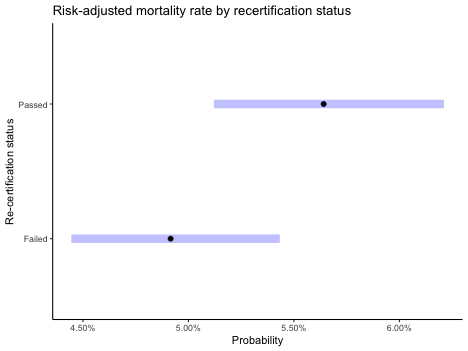
\includegraphics[width=0.75\linewidth]{model_results_files/figure-latex/unnamed-chunk-3-1} \end{center}

\hypertarget{by-procedure}{%
\subsubsection{by procedure}\label{by-procedure}}

top10 most different procedures mortality outcomes by passed vs.~failed
surgeons

\begin{center}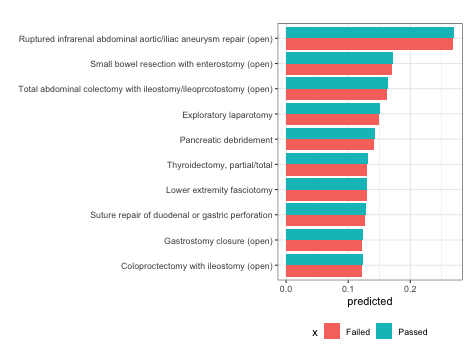
\includegraphics[width=0.75\linewidth]{model_results_files/figure-latex/unnamed-chunk-4-1} \end{center}

\end{document}
